\documentclass[12pt,a4paper]{report}
\usepackage[affil-it]{authblk}
\usepackage{amsthm}
\usepackage{amssymb}
\usepackage{amsmath}
\usepackage{listings}
\usepackage{graphicx}
\usepackage{pgfplots}
\usepackage{float}
\usepackage{xcolor}
\usepackage{hyperref}
\usepackage{algpseudocode}
\usepackage[nameinlink]{cleveref}

\usepackage[
  backend=biber,
  style=alphabetic,
  sorting=anyt,
  minnames=3,
  minalphanames=3
]{biblatex}

\hypersetup{
    colorlinks=true,
    citecolor=blue,
    linkcolor=blue,
    urlcolor=blue,
    pdftitle={Computational Complexity Homework 2024-25},
}

\newtheorem{question}{Question}
\theoremstyle{definition}
\newtheorem{solution}{Solution}

\definecolor{sapRed}{HTML}{6f0a19}
\definecolor{sapBlue}{HTML}{006778}

\newcommand{\curlyquotes}[1]{\textquotedblleft #1\textquotedblright}
\newcommand{\abs}[1]{\left|#1\right|}
\newcommand{\abk}[1]{\left\langle#1\right\rangle}

\addbibresource{./references.bib}

\begin{document}

    \setlength{\parskip}{5pt}               % Vertical spacing between paragraphs
    \setlength{\parindent}{0pt}             % Vertical spacing between paragraphs

    \title{Computational Complexity \\ Homework 2024-25}
    \author{Simone Bianco, 1986936}
    \affil{Sapienza Università di Roma, Italy}
    \date{\today}

    \maketitle

    \begin{question}
        Prove that if $\mathsf{NP} \subseteq \mathsf{BPP}$, then $\mathsf{NP} = \mathsf{RP}$.
        
        To prove this result you may keep in mind that:
        \begin{itemize}
            \item $\mathrm{SAT}$ is self-reducible, this means that you can solve it by reducing to one or more smaller instances of the problem itself.
            \item It is possible, given an algorithm that decides $\mathrm{SAT}$ in polynomial time, to obtain an algorithm that on satisfiable formulas also produces a satisfying assignment.
            \item We saw how to reduce error in probabilistic computation. Essentially, given a polynomial time probabilistic algorithm with two-sided error for $\mathrm{SAT}$,
            you should define another polynomial time probabilistic algorithm for $\mathrm{SAT}$. But this time the algorithm's only errors must be false negatives. And of course the algorithm must have an appropriate probability of success. You have to prove the correctness of your algorithm.
        \end{itemize}
    \end{question}

    \begin{solution}
        First, we observe that the inclusion $\mathsf{RP} \subseteq \mathsf{NP}$ holds without the assumption. Suppose now that that $\mathsf{NP} \subseteq \mathsf{BPP}$. We know that there is a $\mathrm{PDTM}$ $M$ such that:
        \[\abk{\phi} \in \mathrm{SAT} \iff \Pr[M(\phi) = L(\phi)] \geq \frac{2}{3}\]

        where $L(\phi) = 1$ if $\phi \in \mathrm{SAT}$, otherwise $L(\phi) = 0$. Through error reduction, we know that there is a $\mathrm{PDTM}$ $M_p$ that reduces the error of deciding $\mathrm{SAT}$ to less than $\frac{1}{2^{{\abs{\phi}}^p}}$ by repeatedly running $M$, where $p$ is an arbitrary positive constant.
        \[\abk{\phi} \in \mathrm{SAT} \iff \Pr[M_p(\phi) = L(\phi)] \geq 1-\frac{1}{2^{{\abs{\phi}}^p}}\]
        
        We define the following procedure $A$ that constructs a satisfying assignment:

        \begin{algorithmic}[H]
            \Function{$A$}{$\phi$}
                \State Let $\alpha_0$ be an empty partial assignment
                \For{$i$ = $1, \ldots, n$}
                    \If{$M_p(\phi_{\mid \alpha_{i-1} \cup \{x_i = 1\}}) = 1$}
                        \State $\alpha_i = \alpha_{i-1} \cup \{x_i = 1\}$
                    \Else
                        \State $\alpha_i = \alpha_{i-1} \cup \{x_i = 0\}$
                    \EndIf
                \EndFor
                \State Return $\alpha_n$
            \EndFunction
        \end{algorithmic}

        Let $\alpha = A(\phi)$. Suppose that $\phi$ is unsatisfiable. Then, $\alpha$ will never satisfy $\phi$. Hence, we have that:
        \[\abk{\phi} \notin \mathrm{SAT} \implies \Pr[\phi(\alpha) = 1] = 0\]

        Suppose now that $\phi$ is satisfiable. We notice that the assignment returned by the machine is correct not only when all the $n$ calls of $M_p$ give a correct output, but it may also be correct when some (or all) of the calls give the wrong answer. We'll show that restricting our interest to the probability of the case where all the calls accept is sufficient. Let $\mathrm{X_i}$ be the random Bernoulli variable such that $X_i = 1$ if and only if the $i$-th run of $M_p$ inside $A$ is correct. Due to the previous observation, we have that:
        \[\Pr[\phi(\alpha) = 1] > \Pr \left [\bigcap_{i = 1}^n X_i = 1 \right ] = 1 - \Pr \left [\bigcup_{i = 1}^n X_i = 0 \right ]\]

        \textbf{Claim}: For each $n \in \mathbb{N}$, it holds that $\Pr \left [\bigcup_{i = 1}^n X_i = 0 \right ] \leq \sum_{i = 1}^n \Pr \left [ X_i = 0 \right ]$ 

        \begin{proof}[Proof of the claim]
            When $n = 1$, the claim is trivially true. Assume that the claim holds for $n$. With $n+1$ we have that:
            \[\begin{split}
                \Pr \left [\bigcup_{i = 1}^{n+1} X_i = 0 \right ] &= \Pr[X_{n+1} = 0] + \Pr \left [\bigcup_{i = 1}^n X_i = 0 \right ] - \Pr \left [X_{n+1} = 0 \cap \bigcap_{i = 1}^n X_i \right ]\\
                &\leq \Pr[X_{n+1} = 0] + \sum_{i = 1}^n \Pr [X_i = 0 ]
            \end{split} \]
        \end{proof}

        Through the claim we get that:
        \[\Pr[\phi(\alpha) = 1] > 1 - \Pr \left [\bigcup_{i = 1}^n X_i = 0 \right ] \geq 1 -  \sum_{i = 1}^n \Pr \left [ X_i = 0 \right ] \geq 1 - \frac{n}{2^{{\abs{x}}^p}}\]
        which is always greater than $\frac{2}{3}$ for an appropriate choice of $p$. 
        Finally, consider the $\mathrm{TM}$ $M'$ that given $\phi$ in input first computes $A(\phi) = \alpha$ and then returns 1 if and only if $\phi(\alpha) = 1$. By our previous observations we have that:
        \[\abk{\phi} \in \mathrm{SAT} \implies \Pr[M'(\phi) = 1] = \Pr[\phi(\alpha) = 1] \geq \frac{2}{3}\]
        \[\abk{\phi} \notin \mathrm{SAT} \implies \Pr[M'(\phi) = 1] = \Pr[\phi(\alpha) = 1] = 0\]
        Since $M'$ runs in polynomial time, this concludes that $\mathrm{SAT} \in \mathsf{RP}$. Moreover, since $\mathsf{SAT}$ is $\mathsf{NP}$-Complete, this also concludes that $\mathrm{NP} \subseteq \mathrm{RP}$.
    \end{solution}

    \quad

    \hrule

    \quad

    \begin{question} This questions is broken in several tasks.

        \begin{enumerate}
            \item Show a polynomial size branching program for the inner product function
            \[\mathrm{IP}(x_1, \ldots, x_n, y_1, \ldots, y_n) = \sum_{i = 1}^n x_iy_i \pmod{2}\]
            
            \item Given a CNF formula $\phi(x_1, \ldots , x_n)$, describe a branching program that computes $\phi$ of size polynomial with respect to the size of $\phi$. Computing $\phi$ means that the branching program must compute the value of the formula, given as assignment to its variables.
            \item A read-once branching program is one where no variable is queried more than once on any path. Do part 1 again, but with a read-once branching program. Or show that your solution for part one is already read-once.
            \item Can you do a read-once branching program for part 2? If not, why not? Discuss the difficulties, but a formal argument is not required here.
        \end{enumerate}
    \end{question}

    \begin{solution}
        \quad

        \begin{enumerate}
            \item We'll construct a branching program that contains $n$ levels. Each level evaluates the $k$-th sum of the inner product. In particular, each level contains two tracks. The computation will move between the two tracks based on the partial evaluation of the total inner product. To construct the levels, we use three gadgets: a start gadget, a middle gadget and an end gadget.

            \begin{figure}[H]
                \centering
                \begin{tikzpicture}[->,>=stealth,shorten >=1pt,auto,node distance=3cm, thick,]
                    \node [circle, draw](1) []{$x_1$};
                    \node [circle, draw](2) [right of = 1, yshift = -35, ]{$y_1$};

                    \node [circle, draw](3) [below of = 1]{$x_2$};
                    \node [](4) [right of = 3, yshift = -35, ]{};
                    \node [](5) [right of = 4, xshift=50]{};
                    \node [circle, draw](6) [right of = 5, yshift = 35, ]{$x_2$};

                    \path[every node/.style={font=\sffamily\small}]
                        (1) edge node[swap]{0}(3)
                        (1) edge node[swap]{1}(2)
                        (2) edge node[swap]{0}(3)
                        (2) edge node[swap]{1}(6)

                    ;
                    
                \end{tikzpicture}
                \caption{The start gadget}
            \end{figure}

            \begin{figure}[H]
                \centering
                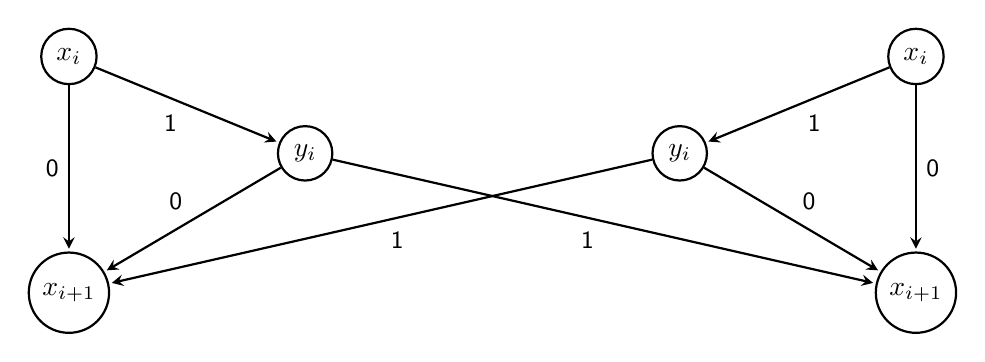
\begin{tikzpicture}[->,>=stealth,shorten >=1pt,auto,node distance=3cm, thick,]
                    \node [circle, draw](3) []{$x_i$};
                    \node [circle, draw](4) [right of = 3, yshift = -35, ]{$y_i$};
                    \node [circle, draw](5) [right of = 4, xshift=50]{$y_i$};
                    \node [circle, draw](6) [right of = 5, yshift = 35, ]{$x_i$};

                    \node [circle, draw](7) [below of = 3]{$x_{i+1}$};
                    \node [circle, draw](10) [below of = 6]{$x_{i+1}$};

                    \path[every node/.style={font=\sffamily\small}]

                        (3) edge node[swap]{0}(7)
                        (3) edge node[swap]{1}(4)
                        (4) edge node[swap]{0}(7)
                        (4) edge node[swap]{1}(10)

                        (6) edge node{0}(10)
                        (6) edge node{1}(5)
                        (5) edge node{0}(10)
                        (5) edge node{1}(7)

                    ;
                    
                \end{tikzpicture}
                \caption{The middle gadget}

            \end{figure}

            \begin{figure}[H]
                \centering
                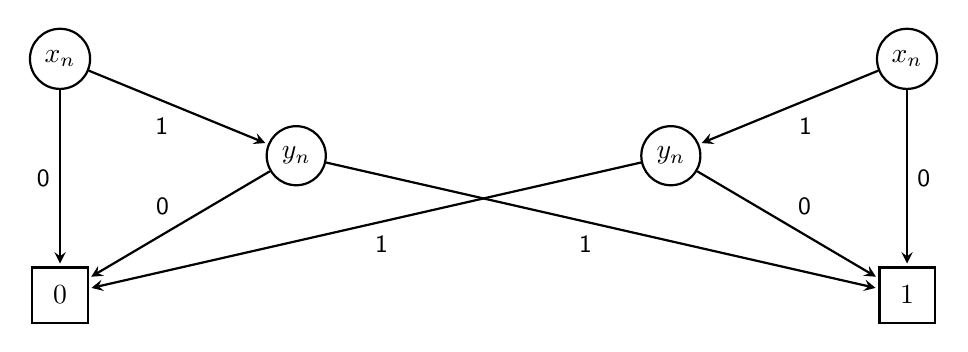
\begin{tikzpicture}[->,>=stealth,shorten >=1pt,auto,node distance=3cm, thick,]
                    \node [circle, draw](11) []{$x_{n}$};
                    \node [circle, draw](12) [right of = 11, yshift = -35, ]{$y_{n}$};
                    \node [circle, draw](13) [right of = 12, xshift=50]{$y_{n}$};
                    \node [circle, draw](14) [right of = 13, yshift = 35, ]{$x_{n}$};

                    \node [rectangle, draw, minimum height = 20, minimum width = 20](15) [below of = 11]{$0$};
                    \node [rectangle, draw, minimum height = 20, minimum width = 20](16) [below of = 14]{$1$};

                    \path[every node/.style={font=\sffamily\small}]

                        (11) edge node[swap]{0}(15)
                        (11) edge node[swap]{1}(12)
                        (12) edge node[swap]{0}(15)
                        (12) edge node[swap]{1}(16)

                        (14) edge node{0}(16)
                        (14) edge node{1}(13)
                        (13) edge node{0}(16)
                        (13) edge node{1}(15)
                    ;
                    
                \end{tikzpicture}
                \caption{The end gadget}
            \end{figure}
            
            Given the input $x_1, \ldots, x_n, y_1, \ldots, y_n$, when $n > 1$, the branching program is constructed by a sequence of $1$ start gadget, $n-2$ middle gadgets and $1$ end gadget. When $n = 1$, the branching program contains a single start gadget, where the two nodes that query $x_{2}$ are replaced by the output nodes 0 and 1. For any $n \in \mathbb{N}$, the size of the constructed branching program is $O(n)$ (see \Cref{bp_1}).
            
            We claim the following invariant to prove the correctness of the program. Once the program reaches the $(n+1)$-th layer, the computation concludes.

            \textbf{Claim}: For any $k \in [n+1]$, if in the $k$-th level the computation starts from the left track, we have that $\sum_{i = 1}^{k-1} x_i y_i \equiv 0 \pmod 2$. Otherwise, if it starts from the right track, we have that $\sum_{i = 1}^{k-1} x_i y_i \equiv 1 \pmod 2$.

            \begin{proof}[Proof of the claim]
                If $k = 1$, we're in the first layer, where we always start from the left track and where the sum is equal to 0. Assume that the claim holds for the $k$-th layer. Assume that the $(k+1)$-th layer starts from the left track (we can use a similar argument for the other case ). Then, this can happen only in two cases:
                \begin{itemize}
                    \item The $k$-th layer started from the left track and $x_k = 0$ or $y_k = 0$. In this case, we have that:
                    \[\sum_{i = 1}^k x_iy_i \equiv x_{k+1}y_{k+1} + \sum_{i = 1}^{k-1} x_iy_i \equiv 0+0 \equiv 0 \pmod 2\]
                    \item The $k$-th layer started from the right track and $x_k = 1$ or $y_k = 1$. In this case, we have that:
                    \[\sum_{i = 1}^k x_iy_i \equiv x_{k+1}y_{k+1} + \sum_{i = 1}^{k-1} x_iy_i \equiv 1+1 \equiv 0 \pmod 2\]
                \end{itemize}
            \end{proof}

            \begin{figure}[H]
                \centering
                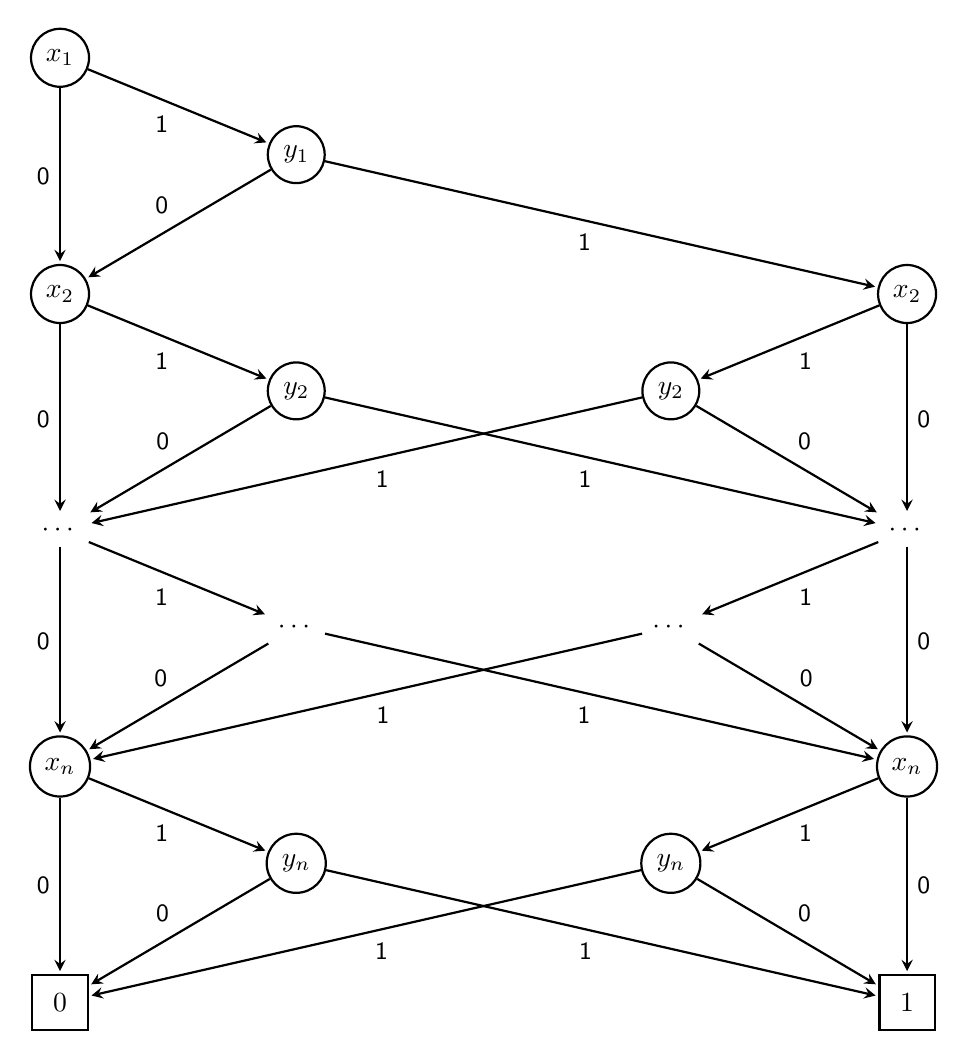
\begin{tikzpicture}[->,>=stealth,shorten >=1pt,auto,node distance=3cm, thick,]
                    \node [circle, draw](1) []{$x_1$};
                    \node [circle, draw](2) [right of = 1, yshift = -35, ]{$y_1$};

                    \node [circle, draw](3) [below of = 1]{$x_2$};
                    \node [circle, draw](4) [right of = 3, yshift = -35, ]{$y_2$};
                    \node [circle, draw](5) [right of = 4, xshift=50]{$y_2$};
                    \node [circle, draw](6) [right of = 5, yshift = 35, ]{$x_2$};

                    \node [](7) [below of = 3]{$\cdots$};
                    \node [](8) [right of = 7, yshift = -35, ]{$\cdots$};
                    \node [](9) [right of = 8, xshift=50]{$\cdots$};
                    \node [](10) [right of = 9, yshift = 35, ]{$\cdots$};

                    \node [circle, draw](11) [below of = 7]{$x_n$};
                    \node [circle, draw](12) [right of = 11, yshift = -35, ]{$y_n$};
                    \node [circle, draw](13) [right of = 12, xshift=50]{$y_n$};
                    \node [circle, draw](14) [right of = 13, yshift = 35, ]{$x_n$};

                    \node [rectangle, draw, minimum height = 20, minimum width = 20](15) [below of = 11]{$0$};
                    \node [rectangle, draw, minimum height = 20, minimum width = 20](16) [below of = 14]{$1$};

                    \path[every node/.style={font=\sffamily\small}]
                        (1) edge node[swap]{0}(3)
                        (1) edge node[swap]{1}(2)
                        (2) edge node[swap]{0}(3)
                        (2) edge node[swap]{1}(6)

                        (3) edge node[swap]{0}(7)
                        (3) edge node[swap]{1}(4)
                        (4) edge node[swap]{0}(7)
                        (4) edge node[swap]{1}(10)
                        
                        (7) edge node[swap]{0}(11)
                        (7) edge node[swap]{1}(8)
                        (8) edge node[swap]{0}(11)
                        (8) edge node[swap]{1}(14)

                        (11) edge node[swap]{0}(15)
                        (11) edge node[swap]{1}(12)
                        (12) edge node[swap]{0}(15)
                        (12) edge node[swap]{1}(16)

                        (6) edge node{0}(10)
                        (6) edge node{1}(5)
                        (5) edge node{0}(10)
                        (5) edge node{1}(7)

                        (10) edge node{0}(14)
                        (10) edge node{1}(9)
                        (9) edge node{0}(14)
                        (9) edge node{1}(11)

                        (14) edge node{0}(16)
                        (14) edge node{1}(13)
                        (13) edge node{0}(16)
                        (13) edge node{1}(15)
                    ;
                    
                \end{tikzpicture}

                \caption{The branching program that computes $\mathrm{IP}(x_1, \ldots, x_n, y_1, \ldots, y_n)$}
                \label{bp_1}
            \end{figure}


            \item Consider the CNF $F = \bigwedge_{i = 1}^m C_j$. For each $j \in [m]$, let $k_j$ be the number of literals in the clause $C_j$, i.e. $C_j = \bigvee_{i = 1}^{k_j} \ell_{i,j}$. We use the following clause gadget to construct the branching program.
            
            \begin{figure}[H]
                \centering

                \resizebox{0.9\hsize}{!}{
                    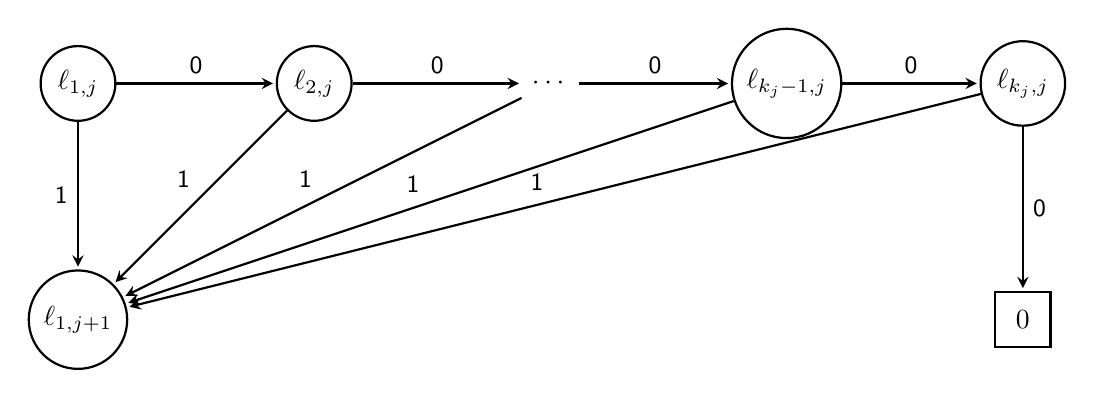
\begin{tikzpicture}[->,>=stealth,shorten >=1pt,auto,node distance=3cm, thick,]
                        \node [circle, draw](1) []{$\ell_{1,j}$};
                        \node [circle, draw](2) [right of = 1]{$\ell_{2,j}$};
                        \node [](3) [right of = 2]{$\cdots$};
                        \node [circle, draw](4) [right of = 3]{$\ell_{k_j-1, j}$};
                        \node [circle, draw](5) [right of = 4]{$\ell_{k_j, j}$};

                        \node [circle, draw](6) [below of = 1]{$\ell_{1,j+1}$};
                        \node [rectangle, draw, minimum height = 20, minimum width = 20](7) [below of = 5]{$0$};

                        \path[every node/.style={font=\sffamily\small}]
                            (1) edge node{0} (2)
                            (2) edge node{0} (3)
                            (3) edge node{0} (4)
                            (4) edge node{0} (5)
                            (5) edge node{0} (7)

                            (1) edge[swap] node{1} (6)
                            (2) edge[swap] node{1} (6)
                            (3) edge[swap] node{1} (6)
                            (4) edge[swap] node{1} (6)
                            (5) edge[swap] node{1} (6)
                        ;
                        
                    \end{tikzpicture}
                }

                \caption{Clause gadget}
            \end{figure}

            \underline{\textbf{Note}}: To make things easier, we're assuming that the branching program can also query the negation of variables. To convert it into standard form, if $\ell_{i,j} = \overline{x_t}$ for some variable $x_t$ then we can simply invert the labels on the edges outgoing from the node labeled with $\ell_{i,j}$.

            Each level of the branching program is the $j$-th clause gadget corresponding to the $j$-th clause of $F$. If $j = m$, the node $\ell_{1,m+1}$ is replaced by the output node 1. For any CNF $\phi$, the branching program has exactly $2+ \sum_{i = 1}^m k_j$ nodes, meaning that the size is linear with respect to the length of $\phi$ (see \Cref{bp_2}). We claim the following property.
            
            \textbf{Claim}: For any $j \in [m]$, the computation on $x$ reaches the node labeled with $\ell_{1,j+1}$ if and only if $C_j$ is satisfied by $x$.

            \begin{proof}[Proof of the claim]
                Suppose that the computation on $x$ reaches the node $\ell_{1,j+1}$. Then, this can only happen if one of the nodes $\ell_{1,j}, \ldots, \ell_{k_j,j}$ takes the edge labeled with 1. Let $\ell_{t',j}$ be such node. Then, this can happen if and only if $\ell_{t',j}$ is set to 1 in $x$.

                Vice versa, suppose that the clause $C_j$ is satisfied by $x$. Let $\ell_{t, j}$ be the first literal of $C_j$ that is set to 1 in $x$. Once the branching program reaches the node $\ell_{t,j}$ it proceeds on the edge labeled with 1, reaching the node labeled with $\ell_{1,j+1}$.
            \end{proof}

            Through the claimed property, we get that the computation on $x$ reaches the output node 1 if and only if $x$ satisfies each clause of $\phi$, proving the correctness of the program.

            \begin{figure}[H]
                \centering

                \resizebox{1\hsize}{!}{
                    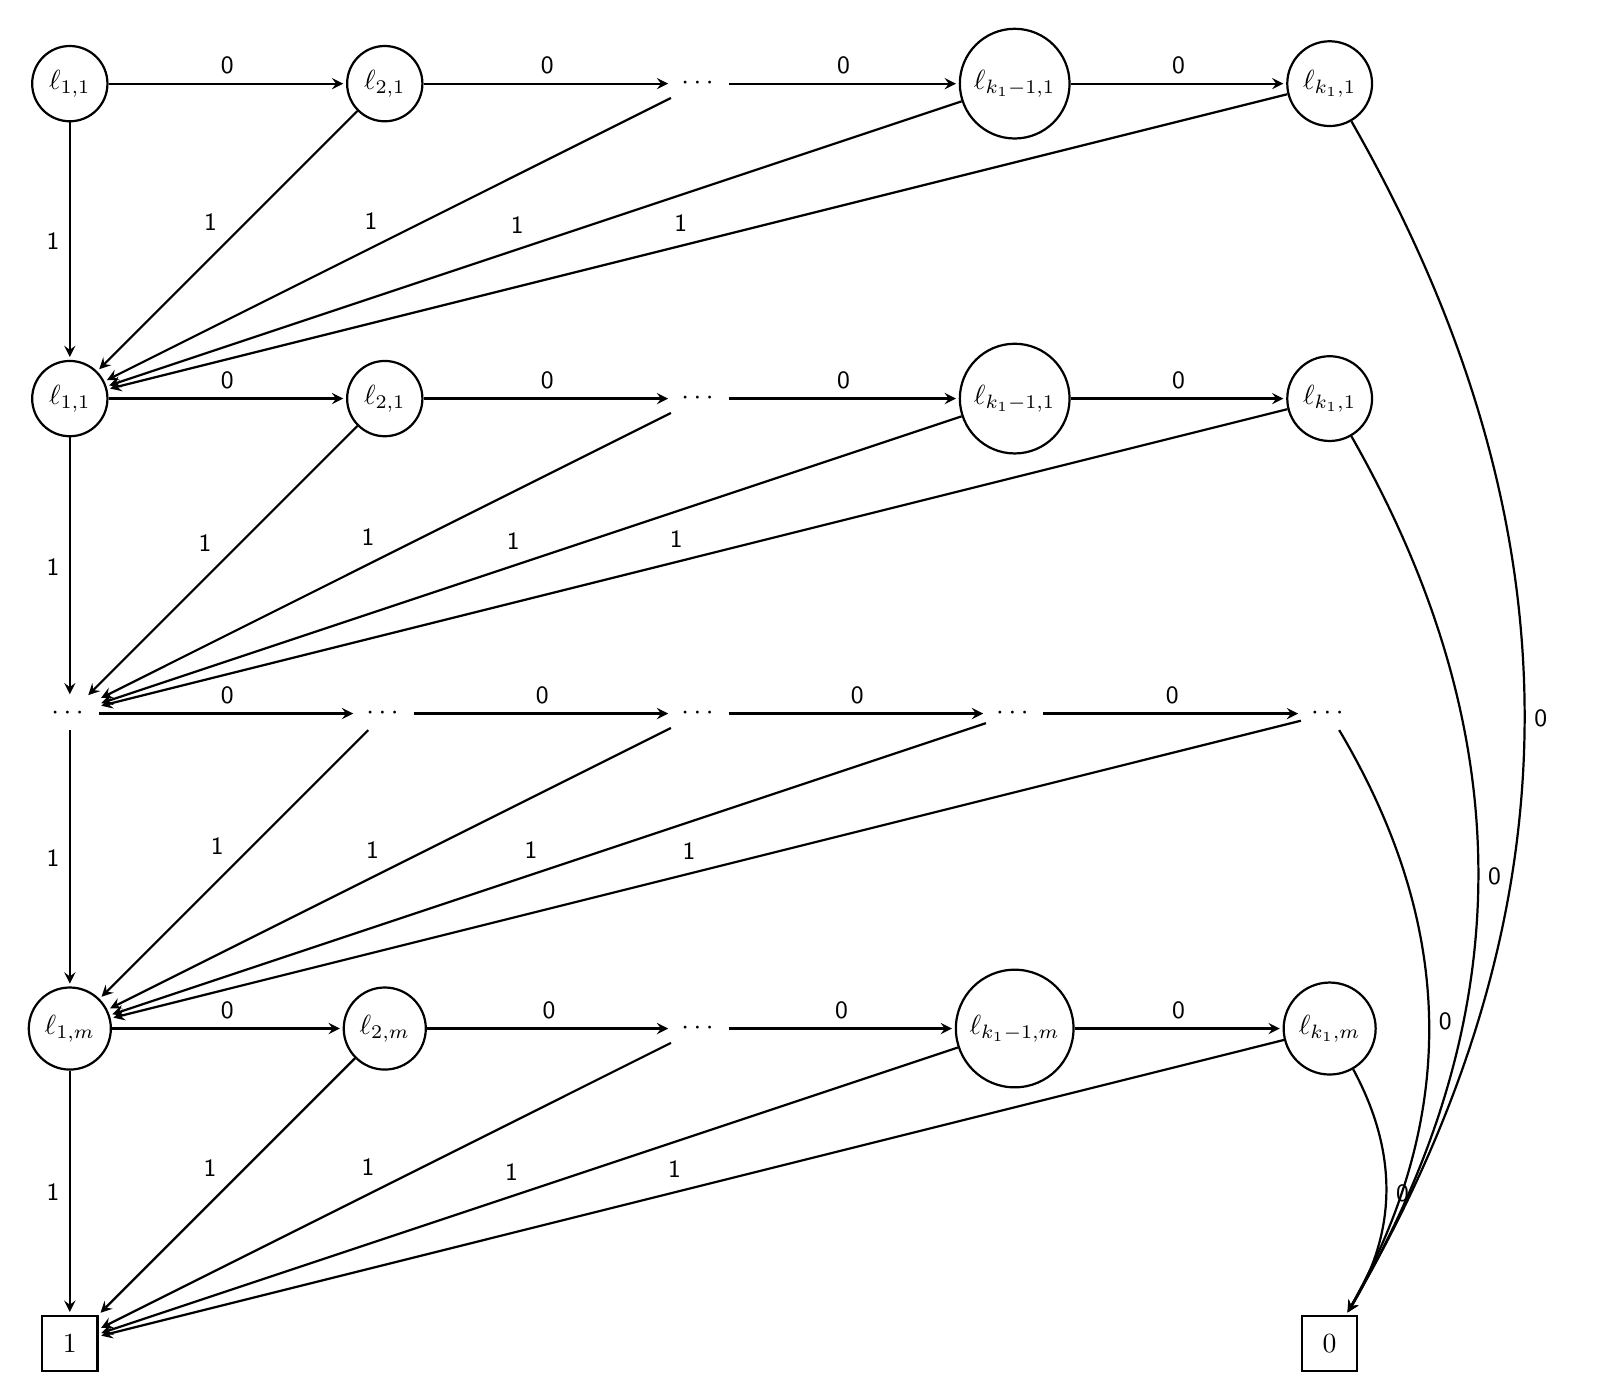
\begin{tikzpicture}[->,>=stealth,shorten >=1pt,auto,node distance=4cm, thick,]
                        \node [circle, draw](1) []{$\ell_{1,1}$};
                        \node [circle, draw](2) [right of = 1]{$\ell_{2,1}$};
                        \node [](3) [right of = 2]{$\cdots$};
                        \node [circle, draw](4) [right of = 3]{$\ell_{k_1-1, 1}$};
                        \node [circle, draw](5) [right of = 4]{$\ell_{k_1, 1}$};

                        \node [circle, draw](6) [below of = 1]{$\ell_{1,1}$};
                        \node [circle, draw](7) [right of = 6]{$\ell_{2,1}$};
                        \node [](8) [right of = 7]{$\cdots$};
                        \node [circle, draw](9) [right of = 8]{$\ell_{k_1-1, 1}$};
                        \node [circle, draw](10) [right of = 9]{$\ell_{k_1, 1}$};

                        \node [](11) [below of = 6]{$\cdots$};
                        \node [](12) [right of = 11]{$\cdots$};
                        \node [](13) [right of = 12]{$\cdots$};
                        \node [](14) [right of = 13]{$\cdots$};
                        \node [](15) [right of = 14]{$\cdots$};

                        \node [circle, draw](16) [below of = 11]{$\ell_{1,m}$};
                        \node [circle, draw](17) [right of = 16]{$\ell_{2,m}$};
                        \node [](18) [right of = 17]{$\cdots$};
                        \node [circle, draw](19) [right of = 18]{$\ell_{k_1-1, m}$};
                        \node [circle, draw](20) [right of = 19]{$\ell_{k_1, m}$};

                        \node [rectangle, draw, minimum height = 20, minimum width = 20](21) [below of = 16]{$1$};
                        \node [rectangle, draw, minimum height = 20, minimum width = 20](22) [below of = 20]{$0$};

                        \path[every node/.style={font=\sffamily\small}]
                            (1) edge node{0} (2)
                            (2) edge node{0} (3)
                            (3) edge node{0} (4)
                            (4) edge node{0} (5)
                            (5) edge[bend left] node{0} (22)
                            (1) edge[swap] node{1} (6)
                            (2) edge[swap] node{1} (6)
                            (3) edge[swap] node{1} (6)
                            (4) edge[swap] node{1} (6)
                            (5) edge[swap] node{1} (6)

                            (6) edge node{0} (7)
                            (7) edge node{0} (8)
                            (8) edge node{0} (9)
                            (9) edge node{0} (10)
                            (10) edge[bend left] node{0} (22)
                            (6) edge[swap] node{1} (11)
                            (7) edge[swap] node{1} (11)
                            (8) edge[swap] node{1} (11)
                            (9) edge[swap] node{1} (11)
                            (10) edge[swap] node{1} (11)

                            (11) edge node{0} (12)
                            (12) edge node{0} (13)
                            (13) edge node{0} (14)
                            (14) edge node{0} (15)
                            (15) edge[bend left] node{0} (22)
                            (11) edge[swap] node{1} (16)
                            (12) edge[swap] node{1} (16)
                            (13) edge[swap] node{1} (16)
                            (14) edge[swap] node{1} (16)
                            (15) edge[swap] node{1} (16)
                            
                            (16) edge node{0} (17)
                            (17) edge node{0} (18)
                            (18) edge node{0} (19)
                            (19) edge node{0} (20)
                            (20) edge[bend left] node{0} (22)
                            (16) edge[swap] node{1} (21)
                            (17) edge[swap] node{1} (21)
                            (18) edge[swap] node{1} (21)
                            (19) edge[swap] node{1} (21)
                            (20) edge[swap] node{1} (21)
                        ;
                    \end{tikzpicture}
                }

                \caption{The branching program that computes $\phi(x_1, \ldots, x_n)$}
                \label{bp_2}
            \end{figure}

            \item The branching program shown in $1.$ is clearly already read-once: each path of each layer queries two different variables and there are no layers that query the same variables.
            
            \item The branching program shown in $2.$ is not read-once. In fact, the whole idea of the solution is to abuse the possibility of querying multiple times the same variables, which may be shared by multiple clauses. This abuse is necessary due to the lack of information regarding how the CNF is structured: if we knew which clauses contained which literals, we could build a read-once program by skipping the literals that have already been queried.
            
            However, even if this were the case, the program would have to split into two sub-programs each time a variable is queried for the first time in order to \curlyquotes{store} the value. Through this process, the size of the program could become exponential.
            
            For instance, if the first clause contains all the variables of the formula then the program would have to split into $2^n$ sub-programs, degenerating into a complete decision tree. 
        \end{enumerate}
    \end{solution}


    \printbibliography


\end{document}